\documentclass{article}

\usepackage[utf8]{inputenc}
\usepackage{float}
\usepackage{booktabs}
\usepackage{titling}
\usepackage{listings}
\usepackage{graphicx}
\usepackage{caption}
\usepackage{subcaption}
\usepackage[margin=0.5in]{geometry}
\usepackage{hyperref}



\title{Predicting Runs}
\author{Derek Owens-Oas, Fan Bu, Federico Ferrari, Megan Robertson}
\date{September 24, 2017}

\begin{document}

\maketitle

\section{Introduction}

We chose to investigate the fourth prompt during the NBA Hackathon - create a model to predict exciting runs during games. One way to define a run is when a team scores on multiple consecutive possessions without the opponent scoring any points in between. This definition captures many runs, but it does not capture the scenario in which a team makes three-pointers on three consecutive possessions, and the other team scores a quiet lay-up in between. We propose a novel and flexible definition of runs which captures scenarios like this. \newline

With runs well defined, we set out with a goal to learn which covariates, or features of the current gameplay, correlate strongly with runs. A few specific hypotheses motivate our analysis. We think there are scenarios in which a streak is more likely. A motivating halftime speech, a large skill differential between the offense?s and defense?s lineups, or an opponent with a propensity to turnover the ball may increase the likelihood of a streak. On the other hand, some features may decrease the likelihood of a run. Playing the second game of a back to back is one example.

\section{Defining an "exciting" run}

In order to make the project approachable during a 24-hour time period, a simplified definition of run was used to classify every possession in the 2016-2017 season. The algorithm below was used to create the labels for the possession log data. 

\begin{figure}[h]
\begin{center}
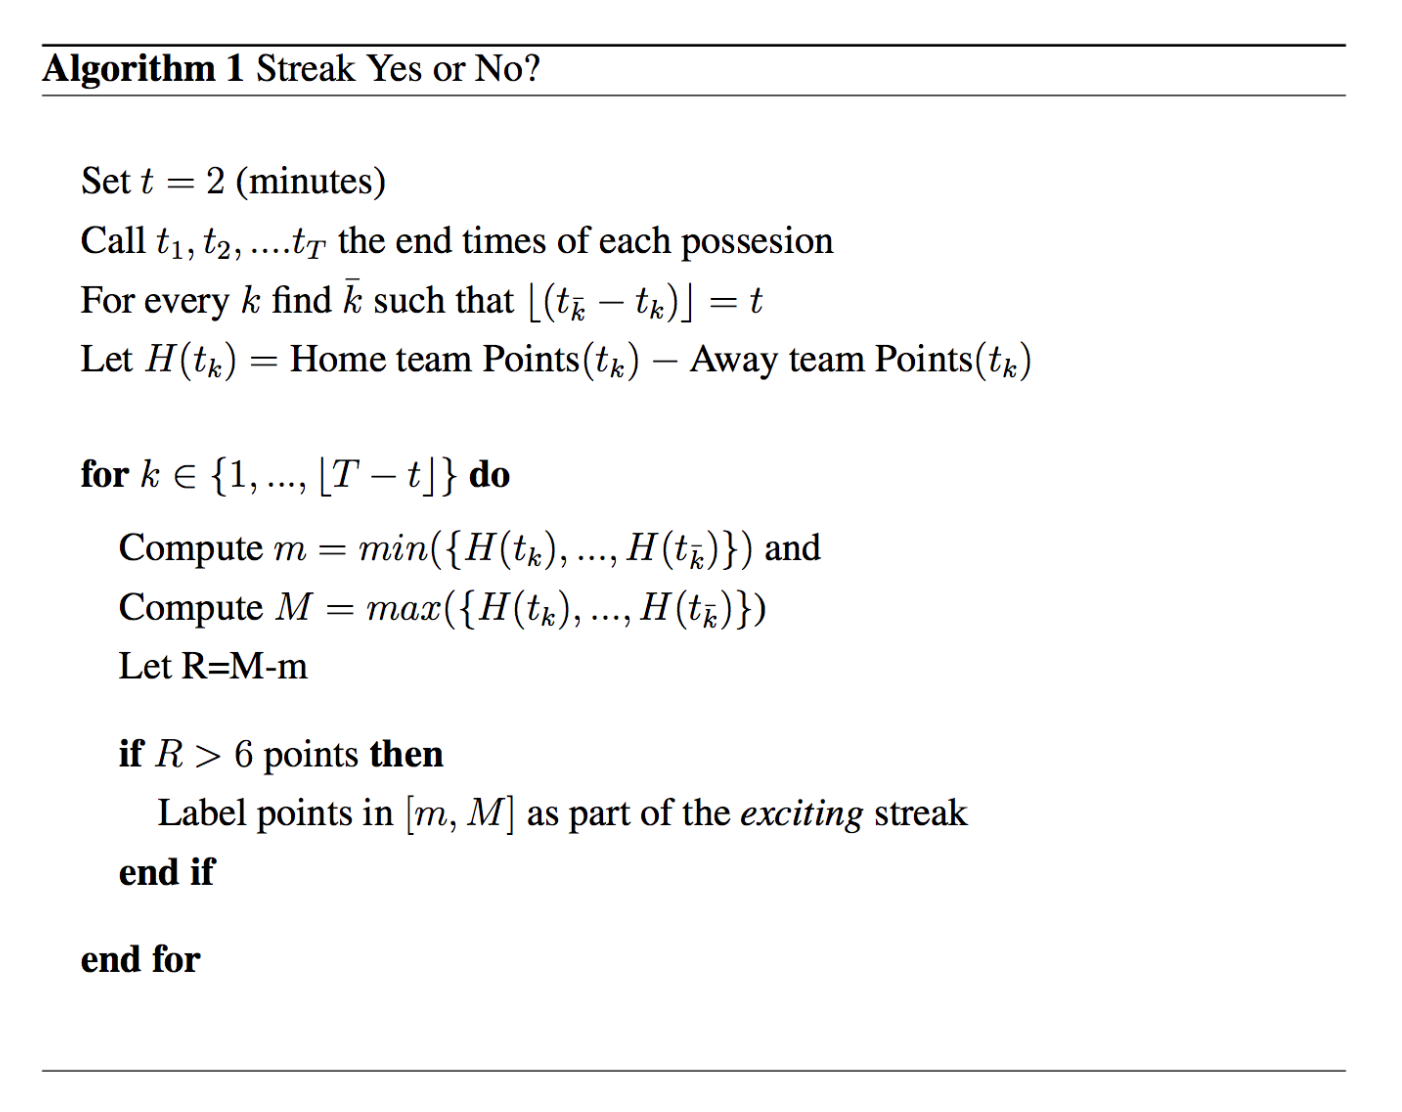
\includegraphics[width=100mm]{alg_screen.png}
\caption{Algorithm for Defining Run}
\end{center}
\end{figure}

The algorithm first finds the interval of length $t$ having as left endpoint the $t_0$, that is the time when the first possession ends. Then, it computes the maximum and the minimum that the function $H()$ attains in the interval, i.e. the highest point difference that we observe in $[t_0,t_0+2]$. We have a run if this point difference exceeds a definite threshold, and if this is the case then we label the points between the Maximum and the minimum as part of the \textit{exiting} streak. Then, we translate the interval and we check $[t_1,t_1+2]$,$[t_2,t_2+2]$, etc. We chose $t$ to be 2 minutes because we wanted to consider exciting,  fast-happening, runs. However, it is clearly possible to $t$ according to different goals. Finally, this choice of $t$ generates around $2-3$ runs per game, so that around 20-30\% of points are labelled as part of a run, making them even harder to detect. 


\section{Feature Generation}

Multiple variables were added to the possession log data that we thought might be indicative of whether a run was occurring at a certain possession in the game.  Two components that define a run are the pace of the game as well as the points being scored. Typically runs are the result of many rapid plays. Therefore, variables were added for the number of shots taken during a possession as well as the number of rebounds. More shots and more rebounds would be indicative of a team getting many offensive boards and having to work for their basket. The type of shot is also very important to consider when exploring runs. Discussions with our coach and other league mentors led us to add an indicator variable defining whether a shot was a "good" shot. This was arbitrarily defined as any shot that was within six feet of the hoop. This is roughly the areas in and around the key closest to the hoop. \newline

In addition to capturing the variability of runs through the above variables, we also wanted to capture the skill level of the players on the court at the time of the run. Using the play by play data, it was possible to determine the players on the court at the time of each possession. From this, we were able to use external data \footnote{"NBA All Star", \url{http://www.nba-allstar.com/players/lists/players-by-draft-pick.html, 9/23/17}} to determine the number of all stars on the court at the time. This is a very basic way to evaluate skill, but other methods could be used to define quality players. However, given the brief work period we only incorporated the all-star information for the time being. 

\section{Modeling Runs}

We approached predicting exciting runs as a classification problem, each possession in a game can either be classified as being part of a run or not. \newline

From a certain team's perspective, each possession has one of 3 potential labels: -1 (an existing run against them), 0 (no existing run), 1 (an existing run favoring them). Therefore we can treat the prediction task as a 3-class classification problem. We propose a multinomial classification model with the label of the next possession as the response and the following variables of the current possession as predictors:\newline

\begin{itemize}
   \item  Period: which period the possession is in (included in the model as a factor)
   \item  Team of possession: which team possesses the ball during that possession
   \item  Net points: the cumulative net point of one of the teams (eg. if that team is losing, this number is negative)
   \item  Rolling net points in the last 3 possessions: the rolling sum of net points won during the past 3 possessions
   \item  Team streak indicator: whether the team with possession is on a run (-1: against; 0: no run; 1: favor)
   \item  Touches
   \item  Dribbles
   \item  Passes
\end{itemize}

We randomly sample 500 games from the 2016-17 season and partition them into 9/1 portions as trainning set and testing set. The model yields a 0.58 top-1 accuracy and 0.86 top-2 accuracy on the test set.\newline

The figures below demonstrate the model prediction results on the game between Golden State Warriors and New Orleans Pelicans on November 7, 2016, when Stephen Curry set a new career record of 3 point shots in one game. \newline

The left plot shows the net point curve of Warriors, with the lighter part as the "runs" detected by our algorithm explained in Section 2. The vertical lines mark the timeouts, with the red ones as timeouts called by the Warriors coach. The dots are the predicted high probability "run" warning points generated by our model, where the orange dots suggest a run favoring the Warriors and the green dots otherwise. It's safe to say that the model is capable of picking up "runs" as defined, since the dots almost perfectly coincide with the highlighted lines. \newline

The right one plots the probability curve assigned to "UP" runs and "DOWN" runs with respect to the Warriors. When the model decides that the Pelicans are going to have a run, the second curve has a peak; otherwise the third curve peaks. We can see very clearly that the peaks of the bottom two curves correspond to the highlighted "runs" in the first plot, where the net points of the Warriors are plotted over the game time.\newline

\begin{figure}[h]
\centering
\begin{subfigure}{.5\textwidth}
  \centering
  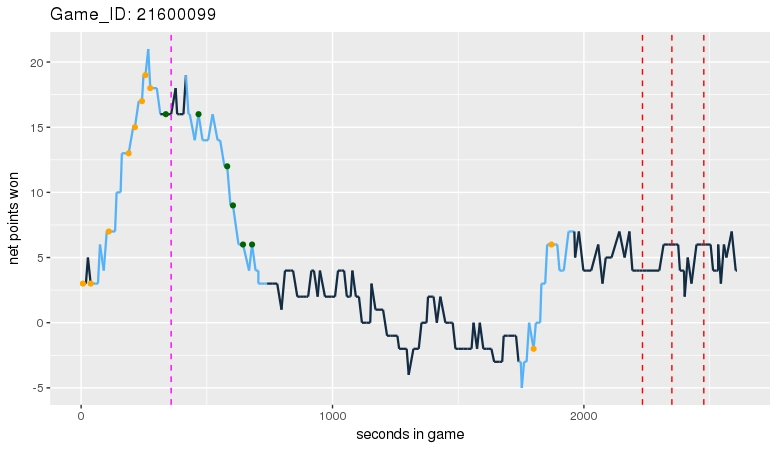
\includegraphics[width=\linewidth]{Net_points_curry.jpeg}
  \label{fig:sub1}
\end{subfigure}%
\begin{subfigure}{.5\textwidth}
  \centering
  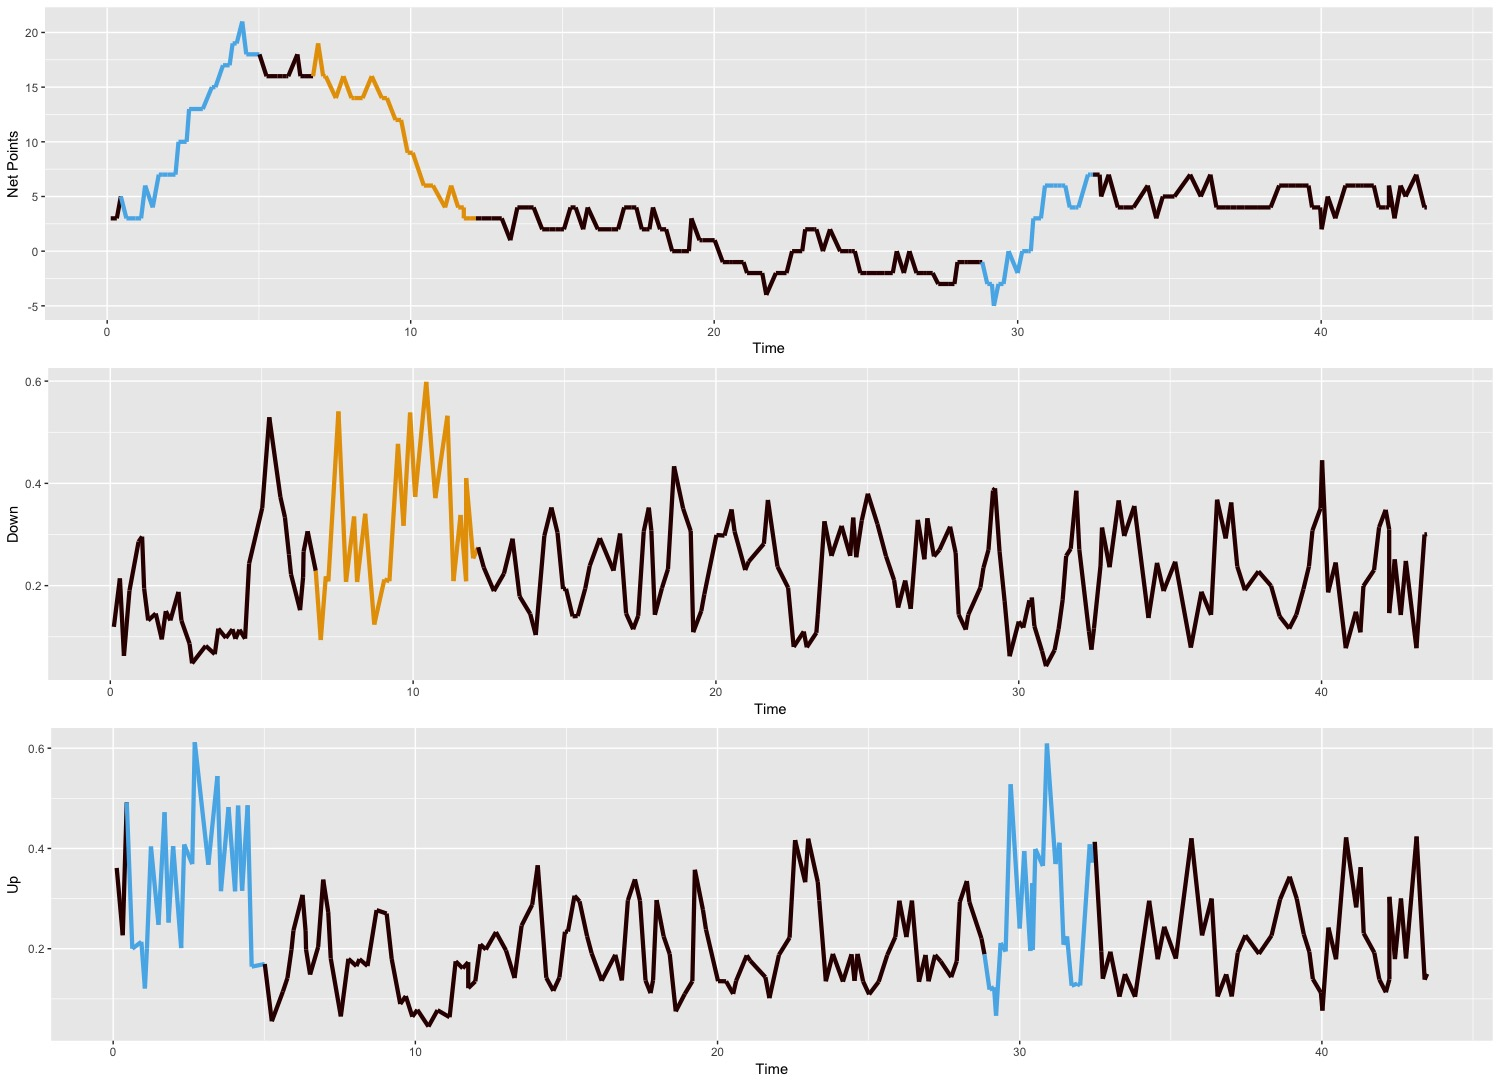
\includegraphics[width=\linewidth]{Pplot2.jpeg}
  \label{fig:sub2}
\end{subfigure}
\caption{Left - Net points curve with timeouts and predictions, Right - UP run and DOWN run probabilities}
\label{fig:test}
\end{figure}



\section{Interpreting Coefficients}

We fit two models, one to predict the probability of going on a run and one for the probability of the opponent going on a run. The plot on the left shows changes in the odds (technically log odds) of going on a run. For example the points coefficient has a positive value. This means for every point scored, we expect an increase in the log odds of approximately $.7$. This agrees with our intuition that higher scoring possessions are more likely to accumulate to a run. In the other direction, we observe a negative effect for a defensive run. There is also a slight significant positive effect for the presence of all stars on the court, confirming intuition that increase in the number of all stars on the court increases the probability of going on a run. On the see predicted changes in the odds of allowing a run. As expected, scoring more points on a possession decreases the odds of allowing a run.

\begin{figure}[h]
\begin{center}
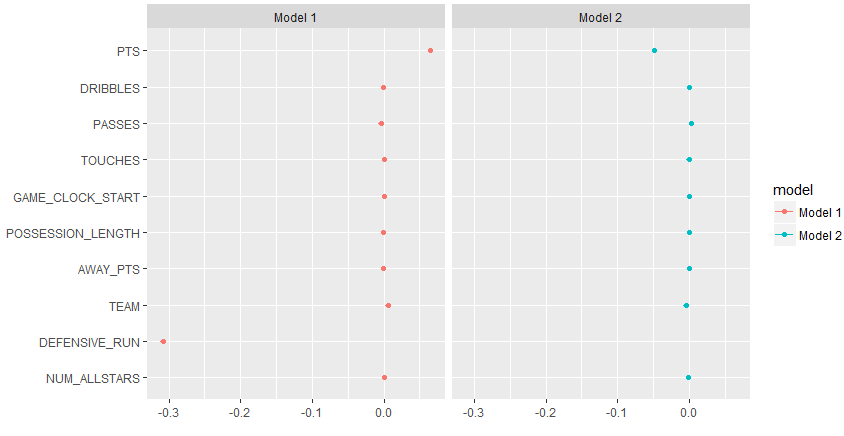
\includegraphics[width=175mm]{results2.png}
\caption{Modeling Results. Model 1 - Odds of going on a run, Model 2 - Odds of allowing a run}
\end{center}
\end{figure}


\begin{figure}[h]
\centering
\begin{subfigure}{.5\textwidth}
  \centering
  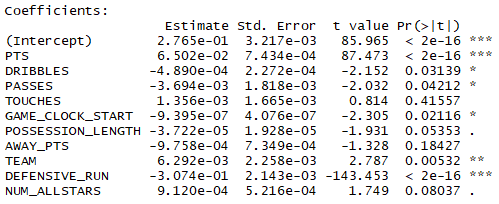
\includegraphics[width=\linewidth]{odds_run_for.png}
  \label{fig:sub1}
\end{subfigure}%
\begin{subfigure}{.5\textwidth}
  \centering
  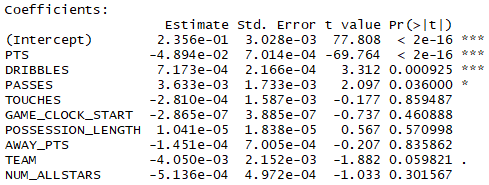
\includegraphics[width=\linewidth]{odds_run_against.png}
  \label{fig:sub2}
\end{subfigure}
\caption{Left - Model 1 Coefficients, Right - Model 2 Coefficients}
\label{fig:test}
\end{figure}

\section{Next Steps}

This project was an attempt to answer a very complex question in a sort period of time. There are a few routes we would consider if we had more time to continue the project. To begin with, there is more data that will most likely capture the variability of whether a possession could be classified as a run. At the moment, the skill of the players is captured by the number of all stars on the court during a possession. However, analyzing different combinations of players, particularly when there are starting players vs. bench players, etc, would be interesting to examine in regards to runs. \newline

Another next step would be to examine different types of classification models. There are many different types of machine learning algorithms that could be implemented in such a project. A more abstract model, such as a decision tree or a support vector machine might capture some of the complicated relationships that are present in the data. 
 

\end{document}
